% !TeX spellcheck = cs_CZ
\wikitextrule
\begin{example}\label{MAI:exam030}
  Je dána funkce \(f: f(x) = \frac{x + 1}{x}\). Sledujme její chování, když hodnoty argumentu \(x\) 
  budou vzrůstat nade všechny meze neboli, jak říkáme, \(x\) se bude blížit k \(+\infty\) (což 
  zapisujeme \(x \to + \infty\) (viz obr. \ref{mai:fig019}). Můžeme psát \(f(x) = 1 + 1/x\). 
  Vzrůstají-li neomezeně hodnoty proměnné \(x\), blíží se hodnoty výrazu \(1/x\) čím dál tím více 
  nule, takže funkční hodnoty \(f(x)\) jsou čím dál tím blíže číslu \(1\). V tomto případě píšeme 
  \(lim_{x\to+\infty} f(x) = 1\) nebo \(f(x) \to 1\) pro \(x\to +\infty\) a říkáme, že funkce \(f\) 
  má v bodě \(+\infty\) limitu rovnou \(1\). Přesně to znamená toto: Zvolíme-li libovolně malé 
  \(\varepsilon > 0\), můžeme nalézt \(p > 0\) tak, že pro \(x > p\) platí \(\abs{f(x) — l} < 
  \varepsilon\). (Viz obr. \ref{mai:fig019}.) Můžeme to říci i takto: Zvolíme-li libovolně okolí 
  bodu \(1\), existuje okolí bodu \(+\infty\) tak, že pro každé \(x\) (konečné) z tohoto okolí je 
  \(f(x)\) ve zvoleném okolí bodu \(1\).
  
  {\centering
   \captionsetup{type=figure}
%   % !TeX spellcheck = cs_CZ

\documentclass[11pt]{standalone}
\usepackage{xltxtra}
\usepackage[usenames,x11names]{xcolor}
\usepackage{tikz}
  \usetikzlibrary{intersections}
  \usetikzlibrary{decorations.markings}
\usepackage{pgfplots}
  \pgfplotsset{compat=newest}
  
\usepackage{amsmath}

\begin{document}
  \begin{tikzpicture}[thick,scale=0.7, 
      every node/.style={transform shape},
      ]
  
  \tikzset{->-/.style={decoration={
    markings,
    mark=at position #1 with {\arrow{stealth}}},postaction={decorate}}}
    
    \begin{axis}[
      xmin = -0.5, xmax = 5.5, ymin = 0, ymax = 4.5,  % osy
      domain =0.2:5,
      restrict y to domain=0:4,
      axis equal image,
      grid = major,   % both
      grid style={line width=.1pt, draw=gray!20},
      major grid style={dashed, line width=.2pt, draw=gray!40},
      clip = true,
      clip mode=individual,
      xtick={1,2,3,4,5}, % make steps of length 0.2
      ytick={0,1,2,3,4}, 
      axis x line = middle,
      axis y line = middle,
      xlabel={$x$}, ylabel={$y$},
      enlarge y limits={rel=0.07},
      enlarge x limits={rel=0.07},
      ]
  
      \addplot[color=Gold3, samples=100, smooth, ultra thick, unbounded coords=jump,
               no markers, domain = 0.1:5, name path global=func1] 
         gnuplot{1+1/x};
  
      \node [fill=white] at (rel axis cs: 0.4,0.75) {\(y=\dfrac{x+1}{x}\)};
  
      \path[name path=line] (0,1.7) -- (3,1.7); 
          % Intersections points
          \path [name intersections={of=func1 and line,by={P1}}] (P1) node [] {};
      
      \draw[black,fill=black] (P1) circle (.3ex);      
      \path (P1 |- 3,-0.1) node [below, fill=white] (X) {p} -- (P1) -- (P1 -| 0,3);
  
      \draw[thick,red, fill=white] ([shift=(90:2.5mm)]X) 
           arc (270:360:1mm) node(Y) {} arc (360:450:1mm);
      \draw[thin] (P1 |- 3,-0.1) -- (P1) -- (P1 -| 0,3);
      \draw[line width = 2pt,red] (Y |- 3,0)  -- ++(3.5,0);
      
   
      \draw[line width = 1pt, black, dashed] (0,1) -- ++(5,0);
      \draw[line width = 3pt, red, line cap=butt] (0,0.3) -- (0,1.7);
      \draw [thick] (-.2, 0.3) node[left] {\(1-\varepsilon\)} -- (0.1, 0.3);
      \draw [thick] (-.2, 1.7) node[left] {\(1+\varepsilon\)} -- (0.1, 1.7 );
  
      \draw[black,fill=white] (0,1) circle (.4ex);

      \path[name path=line] (2.4,0) -- ++(0,2.5); 
          % Intersections points
          \path [name intersections={of=func1 and line,by={P1}}] (P1) node [] {};
          \draw[->-=.4, dashed, gray] (P1 |- 3,-0.05) node[below] {\(x\)} -- (P1);
          \draw[->-=1,  dashed, gray] (P1) -- (P1 -| 0,3) 
            node[left] {\small\(f(x)\)};
            
    \end{axis}
  \end{tikzpicture}
\end{document}
   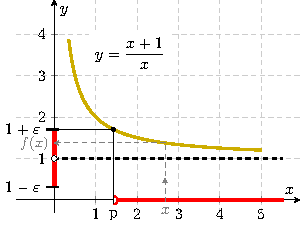
\includegraphics[width=0.45\linewidth]{mai_fig019.pdf}
   \captionof{figure}{K příkladu \ref{MAI:exam030}
   \cite[s.~119]{Brabec1989}
   \label{mai:fig019}}
  \par}
\end{example}















